 \documentclass[a4paper,11pt]{article}
\usepackage[a4paper, total={6in, 10in}]{geometry}
%\documentclass[modern]{aastex631}
\newcommand{\vdag}{(v)^\dagger}
\newcommand\aastex{AAS\TeX}
\newcommand\latex{La\TeX}
\usepackage{romannum}
\usepackage{amsmath}
\usepackage{units}
\usepackage{graphicx}
\usepackage{subfigure}
\usepackage{svg}
\usepackage{natbib}
\usepackage{aas_macros}
\usepackage{caption}
%\usepackage{siunitx}
\PassOptionsToPackage{hyphens}{url}
\usepackage[colorlinks=true, allcolors=blue]{hyperref}
\usepackage{ulem}

\allowdisplaybreaks %To allow long equations to break pages.

\newcommand{\suit}{{\it SUIT}}
\newcommand{\sr}[1]{{\bf\color{red} [#1]}}
\graphicspath{{./}{Figures/}}

%for code environment

\title{RAC Report}
\author{Soumya Roy}
\date{Aug 2023 -- Jan 2024}

\begin{document}

\maketitle

%% ###############################################################
\section{Current Research Work}
%% ##############################################################
I have continued my work for the past six months on the following projects :

%% ###############################################################################
\section*{Project 1: Flare observation}\label{sec3}
%% ###############################################################################

The SUIT is observing flares in Near Ultraviolet (NUV) regime spatially resolved in eleven different science filters, which would let us comment about their overall energy distribution, how the energy release affects the local plasma environment and its long term effect on Earth's atmosphere. In addition to that, we will also gain valuable information about the emission in some specific lines, e.g. Mg II h (279.55 \AA) and k (280.27 \AA), Ca II h (396.85 \AA). We have already started working with preexisting observation in these lines from IRIS and the Helioseismic and Magnetic Imager \citep[HMI;][]{hmi} onboard the Solar Dynamic Observatory \citep[SDO;][]{sdo} in anticipation of what questions we can address with SUIT. The preexisting observations would also help us in testing out the absolute calibration scheme for some of the narrow band channels (NB3,NB4) we proposed during my grad school project.  

The goal was to align the IRIS raster observation with Line of Sight (LOS) magnetic flux density observations from HMI and comment on the role of the magnetic field in flare triggering, the energy distribution and its effect on the local plasma environment. We have studied three different flares (ranging from C class to X class). We have seen a correlated change in local optical depth with the flare light curve, which we believe can be attributed directly to the precipitating flow in the flare loop arms. Figure \ref{fig:optical_dep_ev_m} shows the variation of optical depth in Mg II with respect to the flare light-curve for the \textbf{M3.7} flare that the \textbf{NOAA AR 12443} produced on 4th November 2015. 

Comparing figure \ref{fig:optical_dep_ev_m} shows the GOES X-ray light curve of the event and the variation of the Mg II k and h line intensity ratios as a function of time. The ratio is a standard proxy for plasma optical depth. A value of 2:1 signifies that the plasma is optically thin, while any value lower than that suggests that the plasma is optically thick. Figure \ref{fig:optical_dep_ev_m} shows that the optical depth remains more or less constant during the pre-flare phase. It rises sharply during the impulsive phase, signifying the medium becoming optically thinner due to the flare heating. After that, it sharply decreases again and saturates at a value lower than the pre-flare values. Figure \ref{fig:optical_dep_ev_m} shows that this is during the decaying phase of the flare when the X-ray flux slowly decays, and the precipitation brings a lot of material down into the Chromosphere from the reconnection site. We believe that the medium becomes optically thicker than before due to this rapid influx of material as the density increases very quickly.

%%------------------------%%
\begin{figure}[ht!]
    \centering
    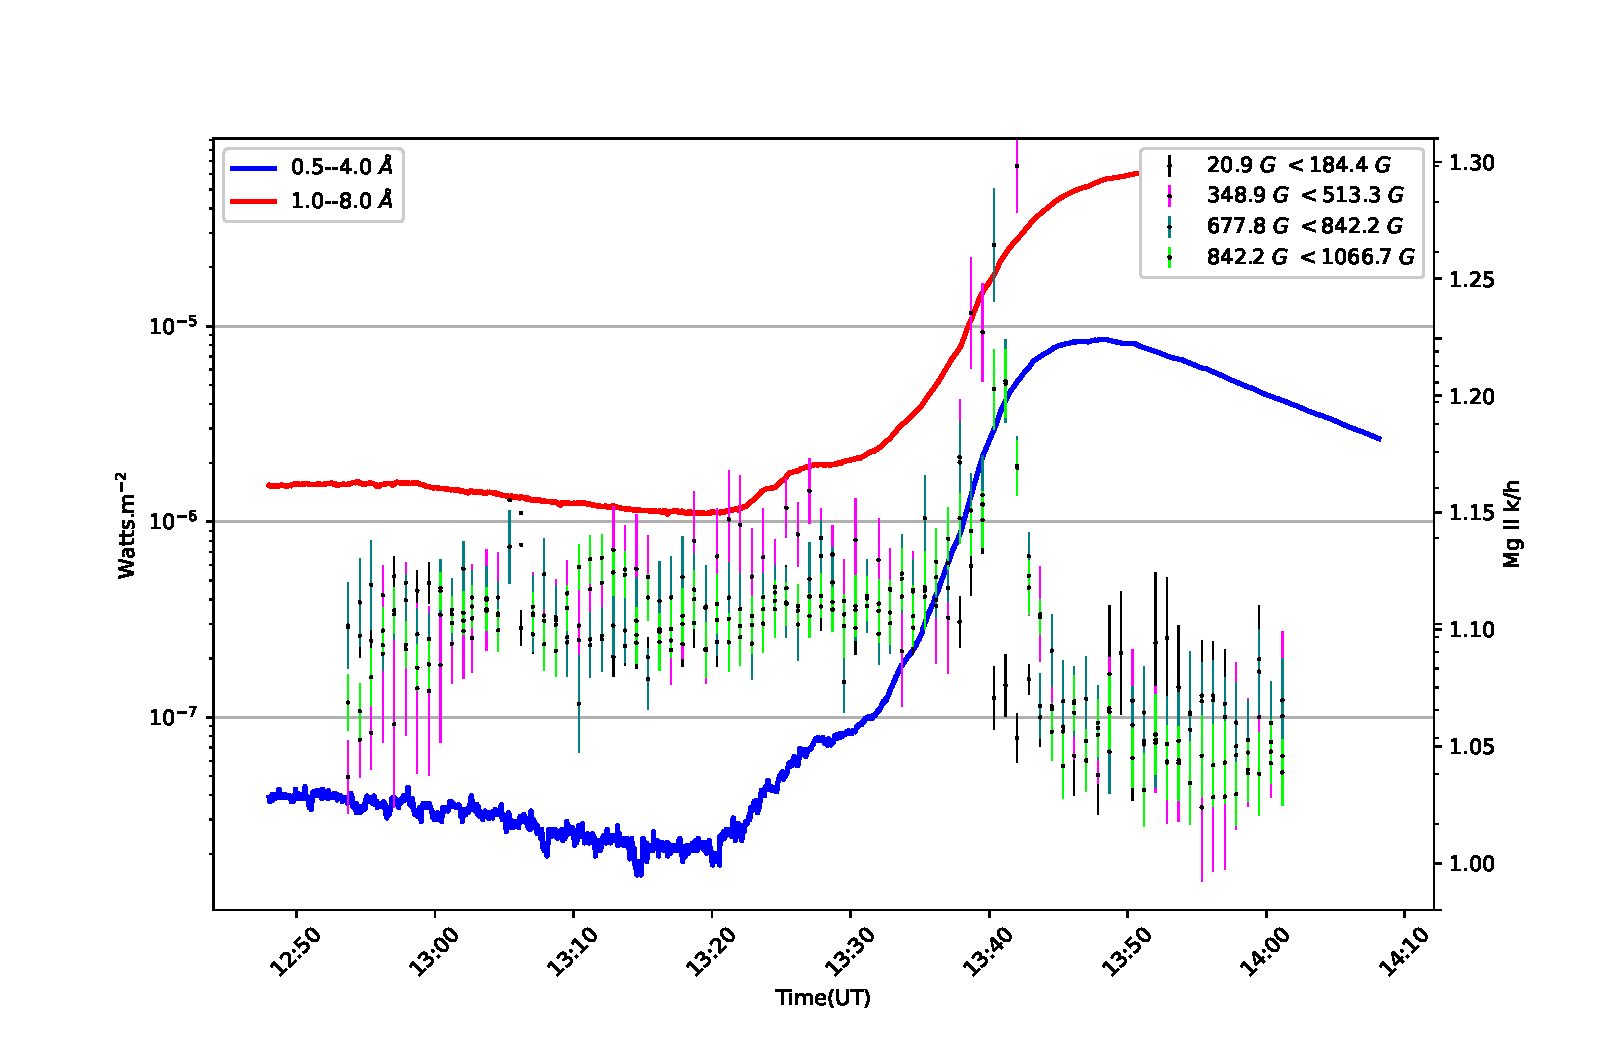
\includegraphics[width=0.8\linewidth]{Figures/Nov-11-2015-optical-dep-ev-3.eps}
    \caption{The figure shows time evolution of the Mg~\Romannum{2} k to h line intensity ratio averaged over all the flaring pixels, in comparison to the GOES flux plot in 0.5{--}4~{\AA} (red) and 1.0~{\AA} (blue).}
    \label{fig:optical_dep_ev_m}
\end{figure}
%%------------------------%%

\textbf{Current status of the project: Submitted to ApJ.}

%% ###############################################################################
\section*{Project 2: Characterizing imaging performance of SUIT}\label{sec2}
%% ###############################################################################

The Solar Ultraviolet Imaging Telescope \citep[SUIT;][]{suit} is an instrument onboard the Aditya L1 mission that will observe the Sun and measure the Solar radiation in the near Ultraviolet range (200-400 nm). SUIT will have the capability of probing various layers of the Sun with its 11 science filters (eight narrow bands and three broad bands). SUIT will provide full-disk and partial disk images of the Sun with a pixel size of 0.7 arcsec. I have been working on various aspects of the instrument characterization for SUIT.

Previously, I had been specifically working on creating an end to end pipeline for creating mock SUIT observations from any MHD simulations of Sun. While that pipeline is in place and working, one of the key components in trying to characterizing the imaging performance is to quantify the effect of the PSF on the imaging, and deconvolving the observed image. This would prove beneficial in scenarios where the pointing of the payload might be off. If the pointing of the payload is not correct, it might result in various portions of the Sun being imaged by the parts of the PSf that distorts the image. This would seriously affect out ability to spatially localize transient impulsive events on the surface of the Sun. We wanted to put a deconvolution pipeline in place that would atleast be able to spatially localize the events more faithfully, even if it is not flux conserving i.e. it would not be very reliable for photometric analysis of the sources. 

We had already studied how the contrast variation across simulated MURaM cubes are reproduced through various filter profiles of SUIT after the PSf convolution. For the NB3 and NB4 filters of SUIT which image the optically thick Mg~\Romannum{2} k and h lines, we had used existing IRIS SJI 2796~\AA~observations in a similar fashion. The final step in this process was to create a preliminary version of the deconvolution pipeline. We have created a working end to end pipeline for deconvolving SUIT observations. To characterize its performance we have used the mock observations we created from existing IRIS observations. In fig.~\ref{fig:deconv} we show the performance of the deconvolution algorithm. In panel a,b \& c we plot the IRIS intensity in the 2832~\AA~continuum, the mock SUIT NB5 observation of the same region and the deconvolved SUIT NB5 observation respectively. In panel d \& e we plot the intensity variation along the white dashed line and blue solid line marked in panel a. The two filaments extending into the sunspot marked by `1' \& `2' in panel a visible along the horizontal blue line, are also marked in panel e. The deconvolved intensity variation shows an enhancement in contrast making the filaments easier to identify. 

%%%%%%%%%%%%%%%%%%%%%%%%%%%%
\begin{figure}[ht!]
    \centering
    \includegraphics[trim={3cm 0cm 4cm 3cm},clip,width=\textwidth]{deconvolve_part_1.pdf}
    \includegraphics[trim={1cm 0cm 1cm 2.8cm},clip,width=\textwidth]{deconvolve_part_2.pdf}
    \caption{Performance of the deconvolution algorithm. \textbf{Panel a:} IRIS raster intensity in 2832~\AA~continuum. \textbf{Panel b:} The IRIS raster observation in \textbf{panel a} convolved with the NB5 PSF. \textbf{Panel c:} The mock SUIT NB5 observation deconvolved with the measured NB5 PSF. \textbf{Panel d (Panel e):} Intensity variation along the white dashed line (blue solid line) for the intnesity normalized IRIS observation(red solid line), mock SUIT NB5 observation (dashed blue line) and deconvolved NB5 observation (green dotted line). The two features marked in panel a,b \& c along the solid blue line are marked in the intensity variation plot.}
    \label{fig:deconv}
\end{figure}
%%%%%%%%%%%%%%%%%%%%%%%%%%%%

We also use a very large dense 320 step raster observation from 20th July, 2023 of a sun spot in AR 13363 to create the mock observation. The sun spot was located at the heliographic position of $\sim [-147",325"]$. The IRIS raster had a filed of view (FoV) $\sim [112",119"]$. As described earlier, we create mock SUIT observation in NB5 passband for this region. In fig.~\ref{fig:nb5_conv_1} panel a we plot the integrated intensity of the IRIS 2832~\AA~window. In panel b we plot the same region passed through the NB5 effective area and convolved with the measured NB5 PSF to create the mock \suit~observation. In panel c (d) we plot a zoomed view of the sunspot in the southern part of the region in IRIS 2832~\AA (mock \suit~NB5 deconvolved). The light bridge in this sunspot goes from a thickness $\sim 1.48\arcsec$ to $\sim 0.75\arcsec$. 


%%%%%%%%-----------------%%%%%%%%%%%%%%%
\begin{figure}[ht!]
    \centering
    \includegraphics[trim={0.3cm 4cm 0 2cm},clip,width=\textwidth]{SUIT_sunspot.pdf}\\
    \includegraphics[trim={0.3cm 3cm 0cm 3cm},clip,width=0.9\textwidth]{SUIT_sunspot_2.pdf}
    \caption{Effects of convolution on the IRIS raster observation with the NB5 PSF. \textbf{Panel (a):} IRIS raster intensity in 2832~\AA continuum.  Multiple small sunspots is marked with white arrows and number `1' to `5'. One bright point is marked with a black arrow and `6'. The two sunspots at the top, marked with '5' and the unnumbered and pointed with white arrow are $\sim$ 1.4" apart. Another larger sunspot with a thin light bridge in the middle is present in the southern part of the region. The light bridge in between the two larger sunspots is marked by a set of four white arrows. The light bridge grows narrower as we move towards south along it. \textbf{Panel (b):} The IRIS raster observation in \textbf{panel a} convolved with the NB5 PSF. \textbf{Panel (c) \& (d):} Zoomed view of the larger sunspot in the South in IRIS and \suit~simulated NB5 map respectively. The light bridge in the middle of the sunspot grows narrower as we travel from north to south. The thickness of the bridge at two different location is marked in both the panels.}
    \label{fig:nb5_conv_1}
\end{figure}
%%%%%%%%-----------------%%%%%%%%%%%%%%%

%%%%%%%%-----------------%%%%%%%%%%%%%%%
\begin{figure}[ht!]
    \centering
    \includegraphics[trim={2cm 3cm 2cm 2cm},clip,width=\textwidth]{SUIT_sunspot_contrast.pdf}
    \caption{\textbf{Top panel:} Cutout of the region marked by dashed red box in fig.~\ref{fig:nb5_conv_1} panel (a). \textbf{Bottom panel:} The normalized intensity along the horizontal blue line from the IRIS and deconvolved mock SUIT observations. The features marked by number `1' to `6' are also marked here.}
\end{figure}
%%%%%%%%-----------------%%%%%%%%%%%%%%%

\textbf{Current status of the project: In preparation}

%%%%%%%%%%%%%%%%%%%%%%%%%%%%%%
\section*{Project 3: Spectral and Photometric characterization of SUIT}
%%%%%%%%%%%%%%%%%%%%%%%%%%%%%%

I also carried out some of the analysis for the photo metric and spectral characterization for the Solar Ultraviolet Imaging Telescope (SUIT). The members of the SUIT team carried out measurements of a standard source to give us estimates of the of spectral characteristics of the SUIT filter combinations. We can also use these measurements to compare our preliminary throughput models with the existing measurements. The standard source was imaged with an optical fiber bundle. After proper background reduction we calculate the 99\% encircled energy from the image to estimate the spatial dispersion of the energy and the total throughput for the standard source. The input energy of the standard source was measured with a photo diode. This allows us to characterize the spectral response of the filter combinations for SUIT.

%%------------------------------%%
\begin{figure}[ht!]
    \centering
    \includesvg[width=0.8\textwidth]{Figures/NB4_spectral_measure.svg}
    \caption{The figure shows the standard source image for the NB4 filter combination at various wavelength within the band imaged through the optical fiber bundle. The encircled energy radius at various wavelength signifies the spatial dispersion of the input energy.}
    \label{fig:nb4-im}
\end{figure}
%%------------------------------%%

%%---------------------------------%%
\begin{figure}[ht!]
    \centering
    \includesvg[width=0.35\textwidth]{Figures/NB2_spectra.svg}
    \includesvg[width=0.35\textwidth]{Figures/NB3_spectra.svg}\\
    \includesvg[width=0.35\textwidth]{Figures/NB4_spectra.svg}
    \includesvg[width=0.35\textwidth]{Figures/NB5_spectra.svg}
    \includesvg[width=0.35\textwidth]{Figures/NB7_spectra.svg}
    \caption{The figure shows the spectral characterization for the SUIT science filter combination. \textbf{Top row:} Measured spectral characteristics for NB2 (left) \& NB3 (right). \textbf{Middle row:} Measured spectral characteristics for NB4 (left) \& NB55 (right). \textbf{Bottom row:} Measured spectral characteristics for NB7.}
    \label{fig:filt-spec}
\end{figure}
%%---------------------------------%%

The same measurements were used to compare the existing throughput model with the expected solar counts for the filter configuration. The throughput model calculates the counts from a standard Sun as a star spectra with $throughput(\lambda)~=~\int~p(\lambda)\times R(\lambda)\times~A\times t~d\lambda$ where $p(\lambda)\implies$ solar photon flux, $R(\lambda)\implies$ the effective wavelength response for a given filter combination, $A\implies$ the collecting area, `t' is the exposure time. 

%%%%%%%%%%%%%%
\begin{tabular}{||c|c|c||}
\hline
    Band Name & Expected counts from measurement & Expected counts from throughput \\
              & (photoelectrons/s) &  (photoelectrons/s) \\
\hline
  NB6 & 105138 & 107064 \\
  NB3 & 18531 & 15520 \\
  NB4 & 35040 & 36717 \\
  NB5 & 124116 & 131625 \\
  NB8 & 26523 & 24096 \\
  NB2 & 53142 & 49099 \\
\hline
\end{tabular}
%%%%%%%%%%%%%%

\textbf{Current status of the project: Waiting for standard star observations from SUIT.}

%% ###################################################### %%
\section*{Project 4(a): Studying Energy Partition in Flares}
%% ##################################################### %%

This project was supported by The NASA Heliophysics System Observatory-Connect (HSO-Connect) program, grant number 80NSSC20K1283 and carried out as a Pre-doctoral fellow in Harvard-Smithsonian Center for Astrophysics as a memeber of the HSO-Connect collaboration.The HSO Connect community comprises GSFC/NASA, NCAR's Whole Heliosphere and Planetary Interactions (WHPI) program and the Parker Solar Probe (PSP) project team at APL (Applied Physics Lab). The purpose of HSO Connect is to unify the community and provide observations coordinated around the PSP mission and other high profile Heliophysics projects requiring unique integration.  

The main goal of my project was to understand how the thermal and Non-thermal energy partition evolves during the evolution of flares, using various available existing solar missions and connecting the data availed from them in our analysis. I have been mainly working on calculating Differential Emission Measure(DEM) maps from Atmospheric Imaging Assembly(AIA) observations for two specific flares, to understand how the thermal energy evolves. The concerned flares are the limb flare which occurred on 29th September, 2020 (Fig. \ref{f_c}) and the X-class flare which occurred on 28th October, 2021 (Fig. \ref{f_d}).

%%------------------------%%
\begin{figure}[h!]
    \centering
    \subfigure[]{\label{f_c}\includegraphics[width=.4\linewidth]{Figures/Flare-2020-11-29.png}}
    \subfigure[]{\label{f_d}\includegraphics[width=.4\linewidth]{Figures/Flare-2021-10-28.png}}
    \caption{The figure \ref{f_c} shows the M-class flare that occurred on the limb and shows very clear magnetic loops rising higher from the surface over the course of its evolution. The figure \ref{f_d} shows the large X-class flare that occurred nearly at the disk center.}
    \label{fig:flares}
\end{figure}
%%------------------------%%

%%------------------------------%%
\subsection*{Thermal Energy}
%%------------------------------%%

Using the Regularised DEM calculator, we have set up the codes capable of calculating DEMs from any sets of observations from any observatory collectively, given they are of the same angular resolution and the temperature response of the concerned pass bands are known. Currently we are mainly using the AIA observations from the six Coronal pass bands (94 \AA, 131 \AA, 171 \AA, 193 \AA, 211 \AA, 335 \AA) to calculate the DEMs. Figure \ref{fig:dem} shows the October flare in its decay phase, and the DEM map calculated at 10.5 MK.

%%------------------------%%
\begin{figure}[h!]
    \centering
    \subfigure[]{\label{d_a}\includegraphics[width=.4\linewidth]{Figures/Flare-2021-10-28-2.png}}
    \subfigure[]{\label{d_b}\includegraphics[width=.4\linewidth]{Figures/Flare-2021-10-28-dem.png}}
    %\includegraphics[width=0.5\linewidth]{Figures/Flare-2020-11-29.png}
    \caption{The figure \ref{d_a} shows the X-class flare in its decay phase and the figure \ref{d_b} shows the DEM map of the same region calculated using the observations six coronal pass-bands of AIA.}
    \label{fig:dem}
\end{figure}
%%------------------------%%

The main goal for calculating the DEM maps is to estimate the thermal energy of the flare. The thermal energy of the flaring plasma is given by $U_{th}~=~3n_{e}k_{B}TfV$, where `V' is the volume of the flaring plasma and `f' is the volume filling factor. As the plasma in our case is multi thermal, we use the calculated DEM to estimate the DEM weighted temperature given by, 

%%------------------------%%
\begin{equation*}
    \bar{T}~=~\frac{\int~DEM(T)T~dT}{\int~DEM(T)~dT}
\end{equation*}
%%------------------------%%

So, for our purpose the the thermal energy is estimated by, 

%%%%%%%%%%%%%%%%%%%%%%%%%%%%
\begin{equation}
    U_{Th}~=~\sum_{j}~\frac{3k_{B}A_{AIA}\sqrt{LOS_{j}}}{\sqrt{EM_{j}}}\int_{T_{min}}^{T_{max}}~DEM(T)_{j}T~dT
\end{equation}
%%%%%%%%%%%%%%%%%%%%%%%%%%%%

where the volume of individual pixel is gievn by $V_{j}~=~A_{AIA}\times~LOS_{j}$, where $LOS_{j}$ is the line of sight (LOS) for the j-th pixel in the FOV and $A_{AIA}$ is the physical area of an AIA pixel, $EM_{j}$ and $DEM(T)_{j}$ are the emission measure in $5<log(T)<7.4$ and the calculated DEM for the j-th pixel in the FOV. We have used the DEM weighted temperature $\bar{T}$ and $n_{e}^{2}\times LOS~=EM$. For our analysis the uncertainty of determining the emitting volume boils down to determining the LOS for individual pixel in the FOV and we have assumed the filling factor to be 1. The only unknown quantity in this equation is the LOS distance, which depends on the geometry of the flare.

%%__________________________________________________________________%%
\subsubsection*{Effects of volume estimation on the thermal energy}
%%__________________________________________________________________%%

One of the main caveats of calculating the total thermal energy from the DEMs is that one can only estimate the volume energy density. To calculate the total thermal energy one needs to estimate the volume of the thermal plasma accurately. As mentioned earlier, for our purpose the concerned volume is the volume of individual AIA pixels given by, $V_{j}~=~A_{AIA}\times~LOS_{j}$. To accurately determine the volume we need to determine the LOS for individual AIA pixels.

We used STEREO-A observations of the event to independently calculate the height of the loops. STEREO-A/EUVI observed the event from a slightly different angle. So, it is possible to triangulate the geometry of the loops. We used co-temporal STEREO 171~\AA,195~\AA~and AIA 171~\AA,193~\AA~images with \textit{scc\_measure.pro}. This routine allows us to select a point on the AIA image. A line representing the LOS from the AIA perspective is then displayed on the EUVI image and vice-versa. According to the emission characteristics, the same point can be identified on the EUVI image. The program determines the 3D coordinates of the point (heliographic latitude, longitude and radial distance). We carry out the same measurement multiple times for various points on the loop top and calculated the average height. Fig.~ \ref{fig:flare_orient} \textbf{a~\&~b} shows the geometric effect of observing from a different vantage. The red cross on fig.~\ref{fig:flare_orient} \textbf{a} shows a point at the top of the flare arcade. The LOS goes into the page through that point from the STEREO-A vantage. The red line in fig.~\ref{fig:flare_orient} \textbf{b} shows the LOS through the point in fig.~\ref{fig:flare_orient} \textbf{a} projected to SDO/AIA point of view.

%%--------------
\begin{figure*}[ht!]
    \centering
    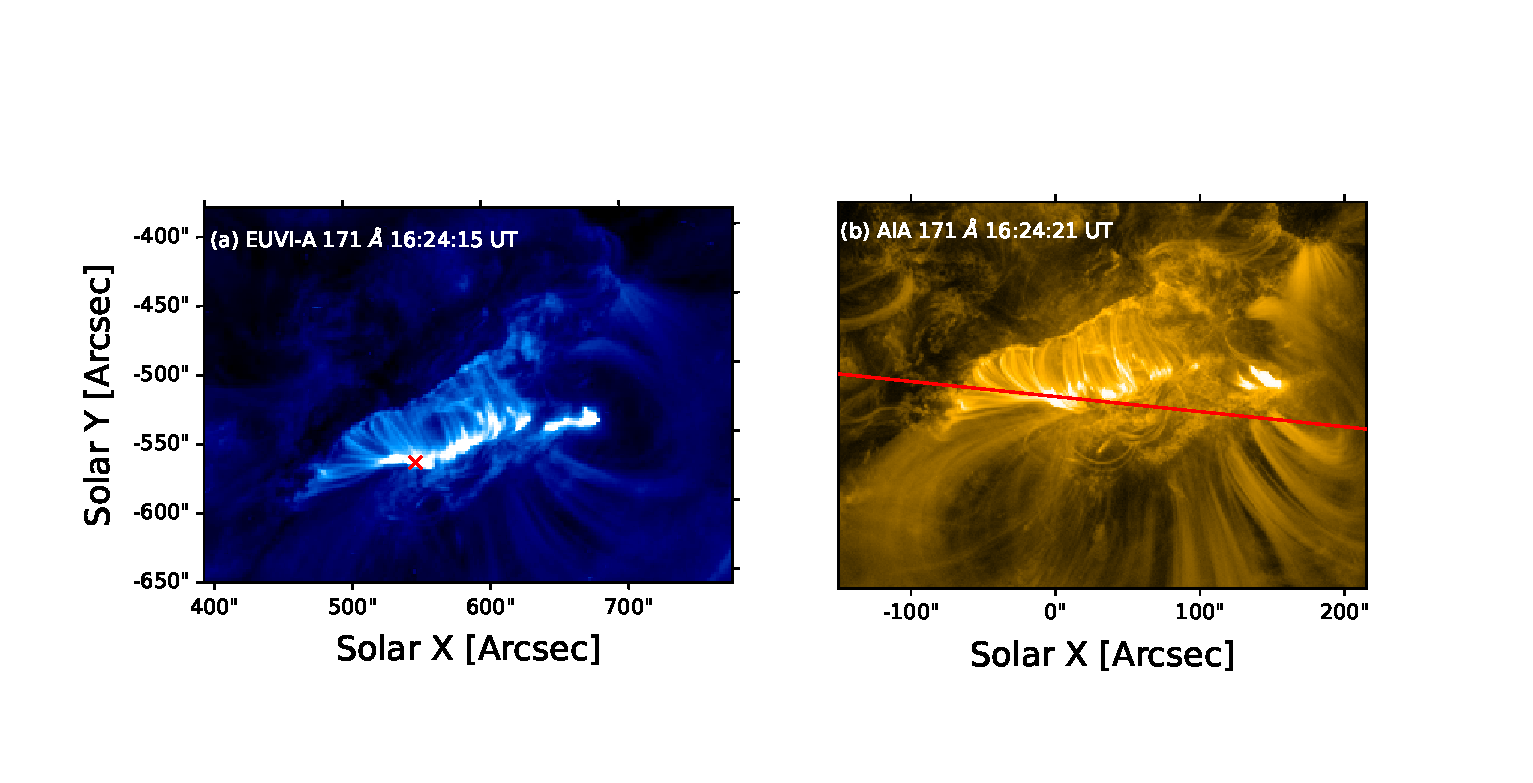
\includegraphics[width=\textwidth,trim={0 0 0 2cm},clip]{Figures/flare_orient.eps} \\
    \hspace{.8cm}
    \raisebox{0.5\height}{\includegraphics[trim={0 0 3cm 1.55cm},clip,width=0.45\textwidth]{Figures/flare_volume_drawing.eps}}
    %\vspace{1cm}
    \raisebox{0.35\height}{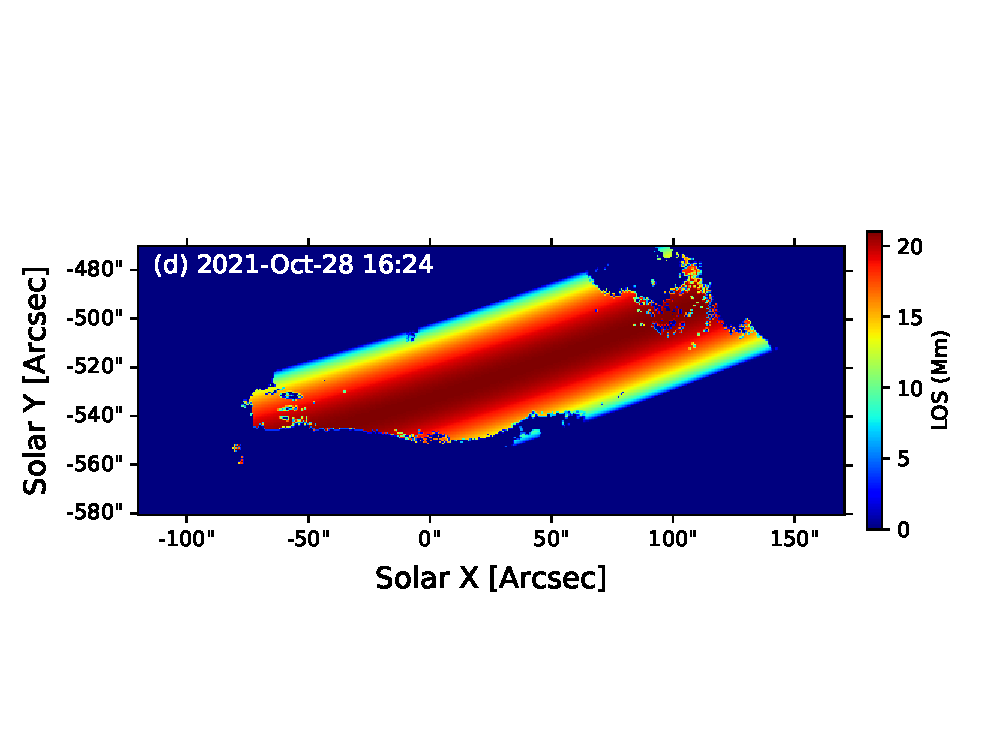
\includegraphics[trim={0 0 0 3cm},clip,width=0.4\textwidth]{Figures/x_flare_los_2.eps}}
    \vspace{-1cm}
    \caption{\textbf{Panel (a):} STEREO-A EUVI 171~\AA~observation of the flare arcade in the decay phase. The red cross marks a point on the top of the arcade. The LOS goes into the page through that point. \textbf{Panel (b):} SDO/AIA 171~\AA observation of the flare arcade. The red line marks the LOS through the arcade from the STEREO-A perspective projected to the AIA perspective. \textbf{Panel (c):} Cartoon demonstrating the projection effects of a semicircular loop between STEREO-A and AIA vantages due to the difference between polar and azimuthal angle respectively. \textbf{Panel (d) :} The calculated LOS map from the AIA perspective, with the calculated loop top height under the assumption of a semi-circular loop geometry.}
    \label{fig:flare_orient}
\end{figure*}
%%--------------

We assumed a semi-circular loop geometry with the height of the loop top to calculate the LOS of every point within the flare arcade.Outside of the flare arcade we assume a LOS~$\sim$~2 Mm (the average thickness of Chromosphere). Unfortunately for most of the duration of this flare the XRT observations are completely saturated. During the impulsive phase of the flare some the EUV channels of AIA are also saturated. We use observations from SUVI when possible. We also use  STIX imaging during the impulsive phase of the flare for the purpose of determining the volume of the flaring plasma.

%%____________________________%%
\subsection*{Non-thermal Energy}
%%____________________________%%

The analysis from the DEMs give us a detailed picture of the thermal component of the energy released from the flares. The energy released from the earlier parts of the flares are mainly dominated by the non-thermal electrons accelerated from the reconncetion site. We plan to quantify the non-thermal energy released using the Fermi, STIX and Chandrayan-XSM data.  We fit the STIX data with a thermal+thick target model for the October 28th flare and the Fermi data for the November 29th event using a thermal+thin target model, as the foot point for the limb event is occulted and the energy from the non-thermal sources would be mainly from the loop top hard X-ray source. The observed photon spectra at Earth is related to the non-thermal electron distribution by the relation,

%------------------------%
\begin{equation*}
    F(\varepsilon)~=~\frac{nNA}{4\pi(AU)^{2}}\frac{1}{mc^{2}}~\int_{\varepsilon}^{E_{eHigh}}~\frac{\sigma(\varepsilon,E)v}{dE/dt}F(E)dE
\end{equation*}
%------------------------%
Where the electron flux distribution is assumed to be isotropic. The figure \ref{g_a} shows a typical fit for STIX spectra.  The figure \ref{g_b} shows the photon distribution observed from the Earth due to the non-thermal component fitted to the spectra. 

%--------------------------%
\begin{figure}[ht!]
    \centering
    \subfigure[]{\label{g_a}\includegraphics[width=0.45\textwidth]{Figures/fit.png}}
    \subfigure[]{\label{g_b}\includegraphics[width=0.45\textwidth]{Figures/photon_dist.png}}
    \caption{The figure \ref{g_a} shows a typical fit to the STIX spectra using a thermal+thick target model. The figure \ref{g_b} shows the resultant photon distribution as observed from the Earth due to the non-thermal accelerated electrons emitting via bremsstrahlung.}
    \label{fig:fit}
\end{figure}
%--------------------------%

\textbf{Current status of the project: Manuscript in preparation}

%%____________________________%%
\section*{Project 4(b): Parker Solar Probe flying through an eruption associated current sheet}
%%____________________________%%

This project is led by HSO-Connect colleagues based in Southwest Research Institute. During Encounter 13, PSP attained a perihelion of 13.3 $\mathrm{R_{\odot}}$. During this time on 5-6th September, 2022 there was a X-class flare appearing on the back side of the Sun. Due tot his, no observatories from Earth was able to register the flare directly. Only Parker Solar Probe (PSP) and Solar Orbiter (SO) had a top down view of the event as they orbit around the Sun. PSP flew through the current sheet emerging from the reconnection. 

We initially went through the Spectrometer/Imaging Telescope for Imaging X-rays (STIX) data onboard the SO data. We created soft X-ray imaging of the region to ensure that PSP was actually flying through the current sheet connected to the same region. We also used the soft X-ray imaging to provide context for the eruption in the lower solar atmosphere, and its energy output to the surrounding atmosphere and how it is connected to the output into the plasma sheet. This also helped us comment about the anorectics of the event and its overall effect on the surrounding plasma. We also used SO 304~\AA and 171~\AA data calculate the footpoint separation rate and infer the ongoing reconnection rate. This will be manifested in observed quantities by PSP while passing the current sheet, such as density, temperature etc.

\textbf{Current status of the project: Manuscript in preparation}

%%%%%%%%%%%%%%%%%%%%%%%%%%%%%%
\section*{Project4(c): Flare energetics working group for SUIT}
%%%%%%%%%%%%%%%%%%%%%%%%%%%%%%

With the successful launch of Aditya-L1 various science questions were posed in the Aditya-L1 Science Working Group (ASWG) along with the initial science goals that can be explored with SUIT, along with other payloads onboard Aditya-L1 and other existing solar missions like SDO/AIA, IRIS etc. Several working groups have been put in place to lead the individual science questions. I am leading the ``Solar flare" working group, specifically focusing on the spectral energy distribution of solar flares in the NUV and investigating the effects of the flares on the local plasma environment from thermal and dynamic evolution of flares. Our association with HSO-Connet collaboration helped us build collaborations with existing solar mission teams.du We have already worked out a initial continiuos observing campaing with IRIS, which would help us with the initial spectral calibration of SUIT NB3, NB4 and NB5.

\textbf{The SUIT team is also putting forward a ``critical science plan" document for the whole mission. The manuscript is in progress.}


%%%%%%%%
\subsection*{Project 5: First X-class flare observed by SUIT}
%%%%%%%%

SUIT was launched in September, 2023 and the first light was on December 8th, 2023. Ever since then it has been continuously observing the sun throughout its cruise phase. It observed the first major X-class flare on Dec 31st, 2023. SUIT observed the flare on east limb of the Sun. In fig.~\ref{fig:aia_evolve} we show the evolution of the flare as seen from AIA. The black field lines are AIA 171~\AA inverted, the violet patches are AIA 1600~\AA inverted and the yellow redd is the AIA 304~\AA. The flare erupts at 21:39 UT launching the loops. A kink in the launched loops develops in 21:42:38 UT. A part of the kink loop starts to accelerate along with the second eruption from the same active region. 

In fig.~\ref{fig:suit_evolve} we plot the observation from the SUIT NB4 aligned with AIA 171~\AA. The bottom panel is AIA 1600~\AA difference images. We can infer the velocity of the ejected structure from the difference maps. The velocity estimate is shown in fig.~\ref{fig:cme_vel}. The blue solid line is the velocity calculated from the AIA 1600~\AA difference maps. The red points is the velocity calculated from the SUIT NB4 observations. The velocities agree well with each other. Due to the larger FOV of SUIT we can calculate the velocity further out. 
The acceleration in the ejected material stars around $\sim$ 21:42 UT as seen from fig.~\ref{fig:cme_vel}. This is consistent with when the kink develops in the ejected loop, i.e. most likely signature of a reconnection. It would be interesting to infer the thermal  of the ejected material from the AIA observations and compare them with observation from XSM, SoLEXS and HEL1OS.

\textbf{Current status of the project: In contact with SoLEXS and HEL1OS team for a coordinated analysis.}

%%---------------------------------%%
\begin{figure}[ht!]
    \centering
    \includegraphics[trim={2cm 2cm 2cm 2cm},clip,width=\textwidth]{Figures/dec31st_evet.pdf}
    \caption{The evoultion of the flare as seen from AIA. The black lines are 171\AA inverted, the violet patches are 1600 \AA inverted and the reddish-yellow is 304\AA. The initial flare erupts at 21:39 UT. The kink in the rising flare arcade develops at 21:42:38 UT. A part of the erupted loops are accelerated along with the second eruption from the second active region.}
    \label{fig:aia_evolve}
    \end{figure}
%%---------------------------------%%

%%---------------------------------%%
\begin{figure}[ht!]
    \centering
    \includegraphics[trim={2cm 2cm 1cm 2cm},clip,width=\textwidth]{Figures/dec31st_evet_ev.pdf}
    \caption{\textbf{Top panel:} The evoultion of the flare as seen from SUIT NB4. The black field lines are 171~\AA inverted. A part of the erupted loops are accelerated along with the second eruption from the second active region. \textbf{Bottom panel:} AIA 1600~\AA difference map. This is used to calculate the velocity of the erupted structure.}
    \label{fig:suit_evolve}
    \end{figure}
%%---------------------------------%%

%%---------------------------------%%
\begin{figure}[ht!]
    \centering
    \includegraphics[width=0.8\textwidth]{Figures/cme_vel.pdf}
    \caption{The velocity of the ejected material as calculated from AIA 1600~\AA and SUIT NB4 observation. The SUIT FOV is bigger compared to AIA, hence we compute the velocity further out.}
    \label{fig:cme_vel}
    \end{figure}
%%---------------------------------%%

%%%%%%%%%%%%%%%%%%%%%%%%%%%%%%



%% #######################################
\section*{List of presentations}
%% #######################################
\begin{enumerate} 
    \item ``Energetics of the November 29th, 2020 limb event" presented in,  \href{https://hinode.nao.ac.jp/hinode16_iris13/#index}{Hindoe-16/IRIS-13}, Niigata, Japan, Sep 2023
    \item ``Thermal and Non-thermal energy evolution in solar flares" presented in, \href{https://www.agu.org/fall-meeting}{AGU 2023}, USA, Dec 2023
    \item ``Solar Ultraviolet Imaging Telescope (SUIT) on-board Aditya-L1", Presented on behalf of the SUIT team in the weekly colloquium of Lockheed Martin Advanced Technology Center, Palo Alto, USA, Dem 2023
\end{enumerate}

\newpage
\bibliography{mybib}{}
\bibliographystyle{aasjournal}

\end{document}
